\scanpage{112}
\(2i=n-1\)\quad i.e. \(i=\dfrac{n-1}{2}\)

induit
\diagram{\begin{array}{ll}A_i^\tau(Y)\ \unsure{\text{---}|\longrightarrow}\ A_i^\tau(X)&\text{surj. exc. }p\end{array}}

\textcircled{3}\quad
\diagram{\begin{tikzcd}[ampersand replacement=\&]A_a^i(X)\arrow[r,"E^{n-2i}"]\&A_a^{n-i}(X)\end{tikzcd}}
\((2i\leq n)\)

\deleted{injectif exc. \(p\)}\inserted{bijectif} mod groupes finis

\deleted{induit \diagram{\begin{array}{ll}A_\tau^i(X)\ \unsure{\text{---}|\longrightarrow}\ A_\tau^{n-i}(X)&\text{bijectif mod groupes finis}\end{array}}}

\diagram{\begin{tikzcd}[ampersand replacement=\&]A_{\deleted{\unsure{\tau|a}}\inserted{r}}^i(X)^\tau\arrow[r,"E^{n-2i+1}"]\&A_r^{n-i+1}(X)^\tau\end{tikzcd}}
\(2i-1\leq n\)

bijectif mod groupes finis

\(\Longrightarrow\)\quad
\diagram{\begin{tikzcd}[ampersand replacement=\&]A_r^i(X)\arrow[r,"E^p"]\&A_r^{i+p}(X)\end{tikzcd}}

a) injectif mod grp finis si \(\unsure{p|r}\leq n-2i\)

b) surjectif mod grp finis si \(p\geq n-2i+1\)
\figure{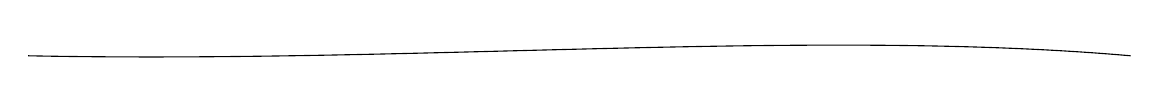
\begin{tikzpicture}\draw(0,0)..controls(5,-.1)and(10,.35)..(14,0);\end{tikzpicture}}
\margin{111}
